\documentclass[11pt]{article}
\usepackage[margin=0.82in]{geometry}
\usepackage{amsmath,amssymb}
\usepackage{booktabs}
\usepackage{graphicx}
\usepackage{float}
\usepackage{array}
\usepackage{enumitem}
\usepackage{xcolor}
\usepackage{listings}
\usepackage{microtype}
\usepackage{fancyhdr}
\usepackage[hidelinks]{hyperref}
\usepackage{caption}

\definecolor{navy}{HTML}{17365D}
\definecolor{lightblue}{HTML}{EAF2F8}
\definecolor{codegray}{HTML}{F4F6F7}
\definecolor{warning}{HTML}{FFF4D6}

\pagestyle{fancy}
\fancyhf{}
\lhead{CSCE 811 -- Homework 2}
\rhead{Nicholas Ampimah}
\cfoot{\thepage}
\setlength{\headheight}{14pt}

\lstset{
  language=Python,
  basicstyle=\ttfamily\footnotesize,
  backgroundcolor=\color{codegray},
  frame=single,
  breaklines=true,
  showstringspaces=false,
  keywordstyle=\color{navy}\bfseries,
  commentstyle=\color{gray},
  columns=fullflexible
}

\newcommand{\todoBox}[1]{%
\begin{center}
\fcolorbox{orange!70!black}{warning}{\parbox{0.92\textwidth}{\textbf{Required before submission:} #1}}
\end{center}}

\title{\textbf{Constructing Temporary Tables for\\Real-Time Combinatorial Quiz Queries}\\[0.4em]
\large CSCE 811 Data Modeling for Systems Development -- Homework 2}
\author{Nicholas Ampimah\\\texttt{<ADD UNL EMAIL>}\\\textit{Add teammate names and emails here, if applicable}}
\date{Fall 2026}

\begin{document}
\maketitle

\todoBox{Replace the email placeholder above and add any teammates before exporting the final submission.}

\begin{abstract}
This project finds every unique combination of four quizzes for which at least $P$ students earned a score of at least $R$ on every quiz. Two general Python algorithms were implemented. Algorithm~1 exhaustively enumerates all $\binom{N}{K}$ quiz combinations and scans the student rows. Algorithm~2 constructs temporary combination levels and stores the intersection of qualifying student sets, pruning an intermediate combination whenever its count falls below $P$. Both programs infer $M$ and $N$ from an arbitrary input CSV and accept $P$, $R$, and $K$ as run-time parameters. On a reproducible $30\times30$ dataset, both methods returned identical results. For $(P,R)=(5,5)$, 1,141 combinations qualified and the median core times were 0.134001240~s and 0.005488753~s for Algorithms 1 and 2, respectively. For $(P,R)=(3,7)$, 268 combinations qualified and the respective median times were 0.137743218~s and 0.002007190~s. Thus, stepwise filtering was 24.41--68.62 times faster in these tests, although both methods retain combinatorial worst-case complexity.
\end{abstract}

\section{Problem Definition and Design Goals}
The input is an $M\times N$ score matrix. Rows represent students, columns represent quizzes, and an entry $a_{sq}$ is the score of student $s$ on quiz $q$. For a candidate quiz set $C$ containing $K$ distinct quizzes, define
\[
\operatorname{count}(C)=\left|\left\{s: a_{sq}\ge R\ \text{for every}\ q\in C\right\}\right|.
\]
The required output is every unordered quiz combination $C$ satisfying $\operatorname{count}(C)\ge P$, together with its count. Using combinations instead of permutations ensures that, for example, $(Q1,Q2,Q3,Q4)$ and $(Q2,Q1,Q3,Q4)$ are not both reported.

The implementation goals were correctness on arbitrary compatible CSV files, no external database, flexible $P$, $R$, and $K$, deterministic output order, explicit validation, comparable timing, and identical output formats for both algorithms.

\section{Step 1: Random Data Generation}
The script \texttt{data\_generate.py} uses NumPy's reproducible random-number generator. The report experiments used $M=N=30$, integer scores from 0 through 10, and seed 811. Student IDs are \texttt{S1}--\texttt{S30}; quiz IDs are \texttt{Q1}--\texttt{Q30}. The CSV preserves the student IDs in its first column.

\begin{lstlisting}
rng = np.random.default_rng(seed)
scores = rng.integers(0, 11, size=(rows, columns))
df = pd.DataFrame(scores,
    index=[f"S{i}" for i in range(1, rows + 1)],
    columns=[f"Q{i}" for i in range(1, columns + 1)])
df.index.name = "student_id"
df.to_csv(output)
\end{lstlisting}

\begin{figure}[H]
  \centering
  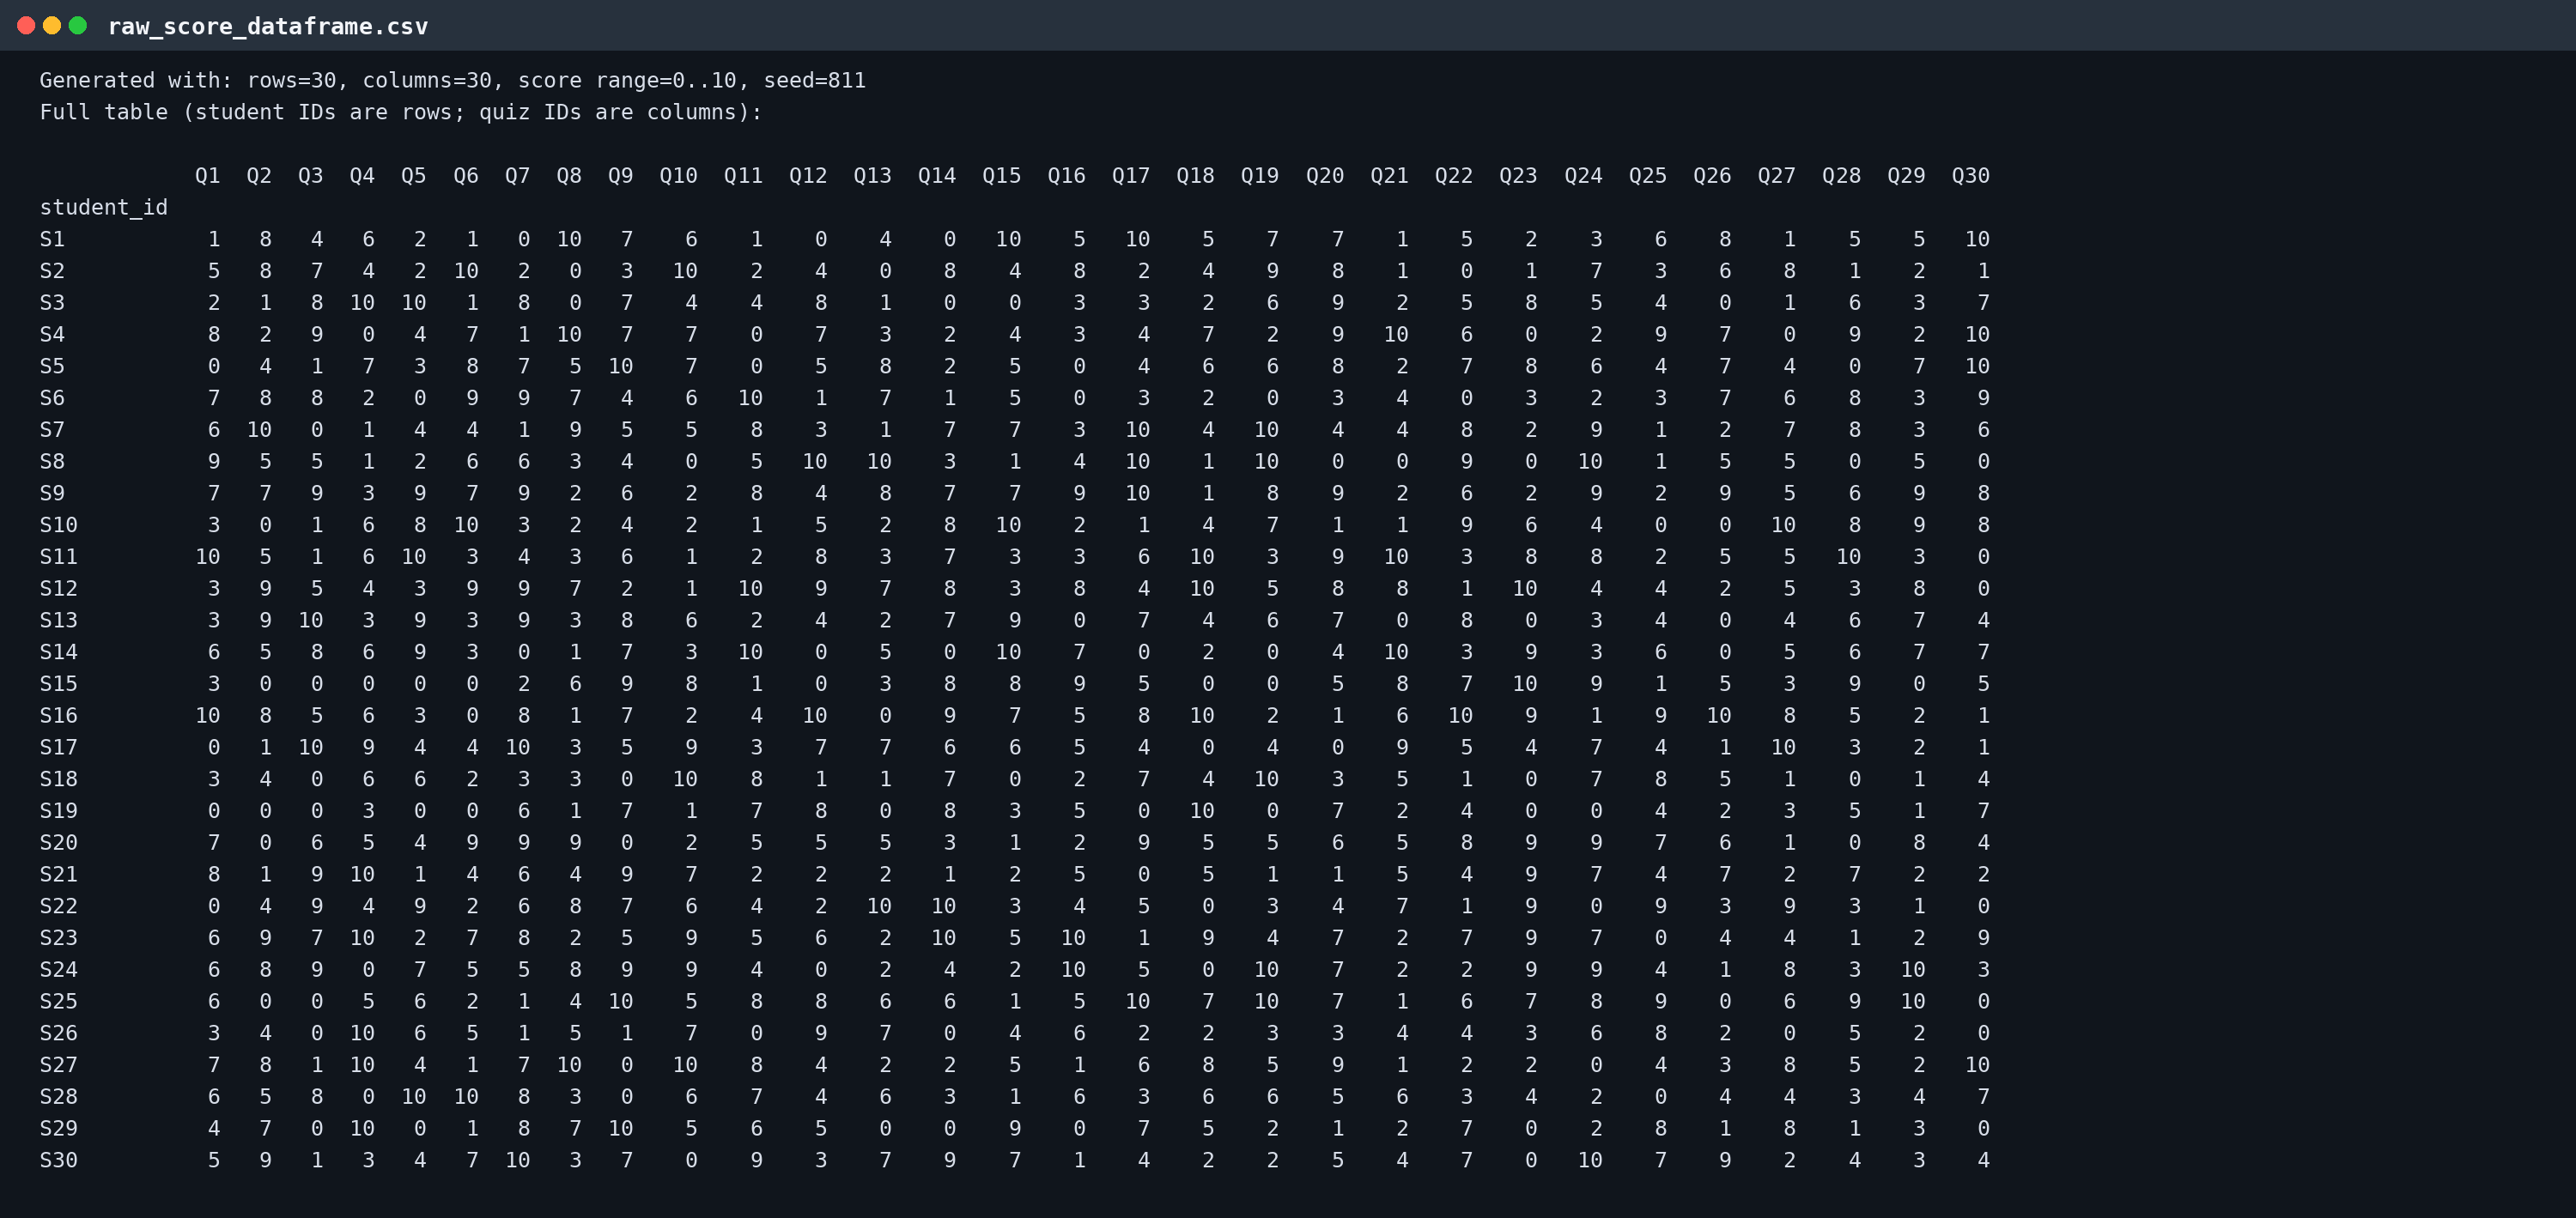
\includegraphics[width=\textwidth]{../report_assets/generated_data.png}
  \caption{The complete reproducible $30\times30$ score dataframe generated with seed 811.}
\end{figure}

\section{Step 2: Algorithm Implementations}

\subsection{Algorithm 1: exhaustive combination enumeration}
Algorithm~1 converts the score matrix into a Boolean matrix using the threshold $a_{sq}\ge R$. It then obtains every size-$K$ column combination with \texttt{itertools.combinations}. For each combination, it applies a row-wise logical AND across the selected columns and counts the \texttt{True} rows. Results with counts at least $P$ are written to CSV.

\begin{lstlisting}
for indices in itertools.combinations(range(len(quiz_ids)), k):
    count = int(np.all(passing[:, indices], axis=1).sum())
    if count >= p:
        results.append((tuple(quiz_ids[i] for i in indices), count))
\end{lstlisting}

This method is a direct implementation of the problem definition and provides a useful correctness baseline.

\subsection{Algorithm 2: stepwise filtering with temporary structures}
Algorithm~2 first creates a temporary mapping from each quiz to the set of student positions whose scores meet $R$. It retains only singleton quizzes with at least $P$ students. At level $d$, every retained $(d-1)$-tuple is extended only by quizzes occurring after its last quiz in the original column order. The stored student set is intersected with the new quiz's set; the new tuple is retained only if the intersection contains at least $P$ students. This continues from level 1 through level $K$:
\[
(Q_i)\longrightarrow(Q_i,Q_j)\longrightarrow\cdots\longrightarrow(Q_{i_1},\ldots,Q_{i_K}).
\]

\begin{lstlisting}
for combination, students in level:
    last_position = order[combination[-1]]
    for next_position in range(last_position + 1, len(quiz_ids)):
        next_quiz = quiz_ids[next_position]
        common_students = students.intersection(eligible[next_quiz])
        if len(common_students) >= p:
            next_level.append((combination + (next_quiz,), common_students))
\end{lstlisting}

The pruning rule is correct because intersection is anti-monotone. If $C\subset C'$, then the students passing every quiz in $C'$ are a subset of those passing every quiz in $C$:
\[
S(C')=\bigcap_{q\in C'}S(q)\subseteq\bigcap_{q\in C}S(q)=S(C).
\]
Therefore, once $|S(C)|<P$, no extension of $C$ can later reach $P$. Extending only in increasing column order also prevents redundant permutations.

\subsection{Input handling and output structure}
Both programs read the first CSV column as student IDs, infer $M$ and $N$, require unique student and quiz IDs, require numeric nonmissing scores, and validate $P\ge1$ and $1\le K\le N$. A value $P>M$ is allowed and correctly produces an empty result. Both output the schema
\[
\texttt{quiz\_1, quiz\_2, \ldots, quiz\_K, count}.
\]

\section{Step 3: Testing and Results}

\subsection{Reproduction instructions}
From the unzipped code directory, install the two dependencies and run:

\begin{lstlisting}[language=bash]
python -m pip install -r requirements.txt
python data_generate.py --rows 30 --columns 30 --seed 811 \
  --output raw_score_dataframe.csv

python algorithm1.py raw_score_dataframe.csv 5 5 --k 4 \
  --output algorithm1_results.csv
python algorithm2.py raw_score_dataframe.csv 5 5 --k 4 \
  --output algorithm2_results.csv

python run_experiments.py
python test_algorithms.py
\end{lstlisting}

The first positional value after the CSV is $P$, the second is $R$, and \texttt{--k} selects the number of quizzes. The main experiment repeats each algorithm seven times and reports the median core time to reduce the effect of transient system activity. File reading and output writing are excluded from the core query timing for both algorithms. The regression test additionally compared both methods across 100 combinations of random seed, $P$, $R$, and $K$; every output matched exactly.

\subsection{Observed results}
\begin{table}[H]
\centering
\caption{Median core runtimes over seven repetitions on the seeded $30\times30$ dataset.}
\begin{tabular}{ccccrrr}
\toprule
Case & $P$ & $R$ & Matches & Algorithm 1 (s) & Algorithm 2 (s) & Speedup \\
\midrule
1 & 5 & 5 & 1,141 & 0.134001240 & 0.005488753 & 24.41$\times$ \\
2 & 3 & 7 & 268 & 0.137743218 & 0.002007190 & 68.62$\times$ \\
\bottomrule
\end{tabular}
\end{table}

\begin{table}[H]
\centering
\caption{Number of Algorithm 2 combinations retained at each temporary level.}
\begin{tabular}{crrrr}
\toprule
Case & 1-quiz & 2-quiz & 3-quiz & 4-quiz \\
\midrule
1: $(P,R)=(5,5)$ & 30 & 420 & 1,506 & 1,141 \\
2: $(P,R)=(3,7)$ & 30 & 326 & 522 & 268 \\
\bottomrule
\end{tabular}
\end{table}

Although Case 1 has the larger $P$, its lower score threshold $R=5$ leaves more students in each quiz set and therefore more intermediate combinations. Case 2 has a higher score threshold, so its student sets shrink earlier and the pruning advantage is larger.

\begin{figure}[H]
  \centering
  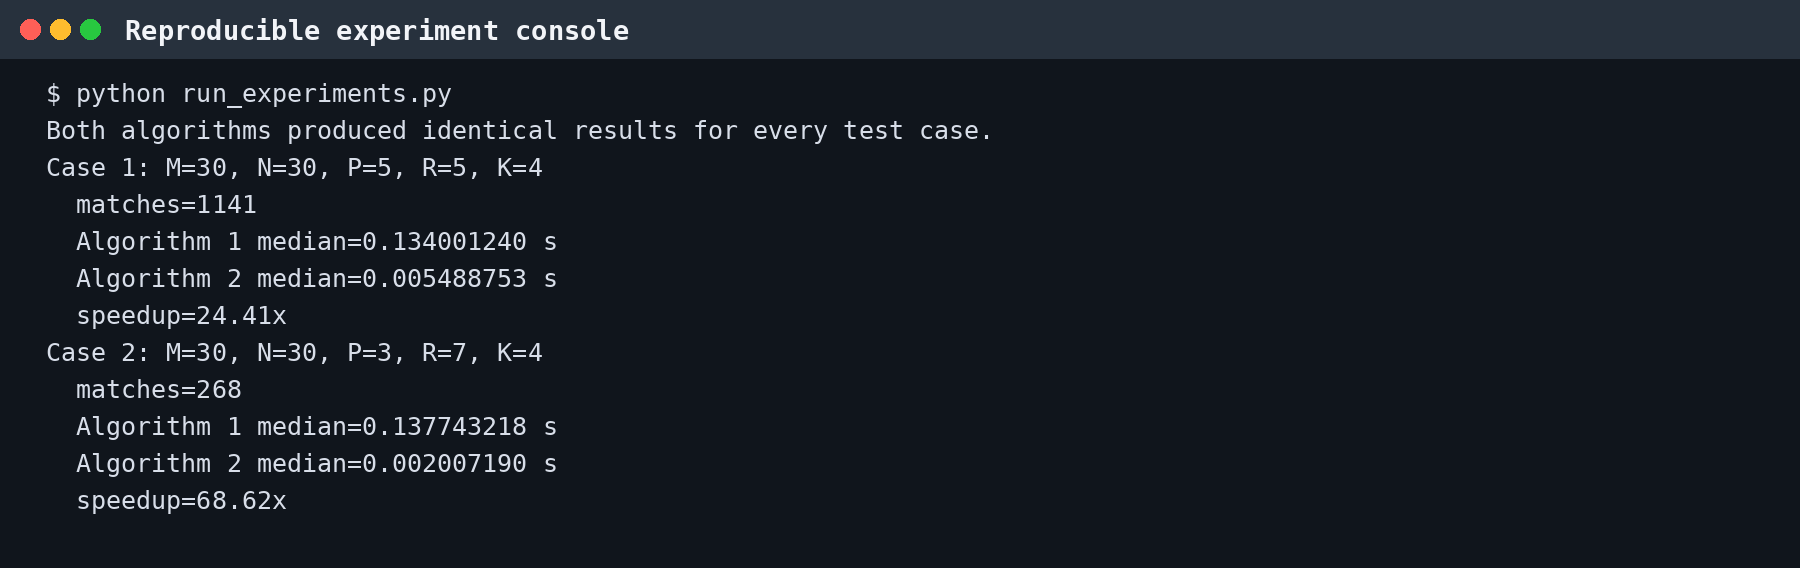
\includegraphics[width=0.96\textwidth]{../report_assets/runtime_console.png}
  \caption{Console evidence from the reproducible two-case experiment.}
\end{figure}

\begin{figure}[H]
  \centering
  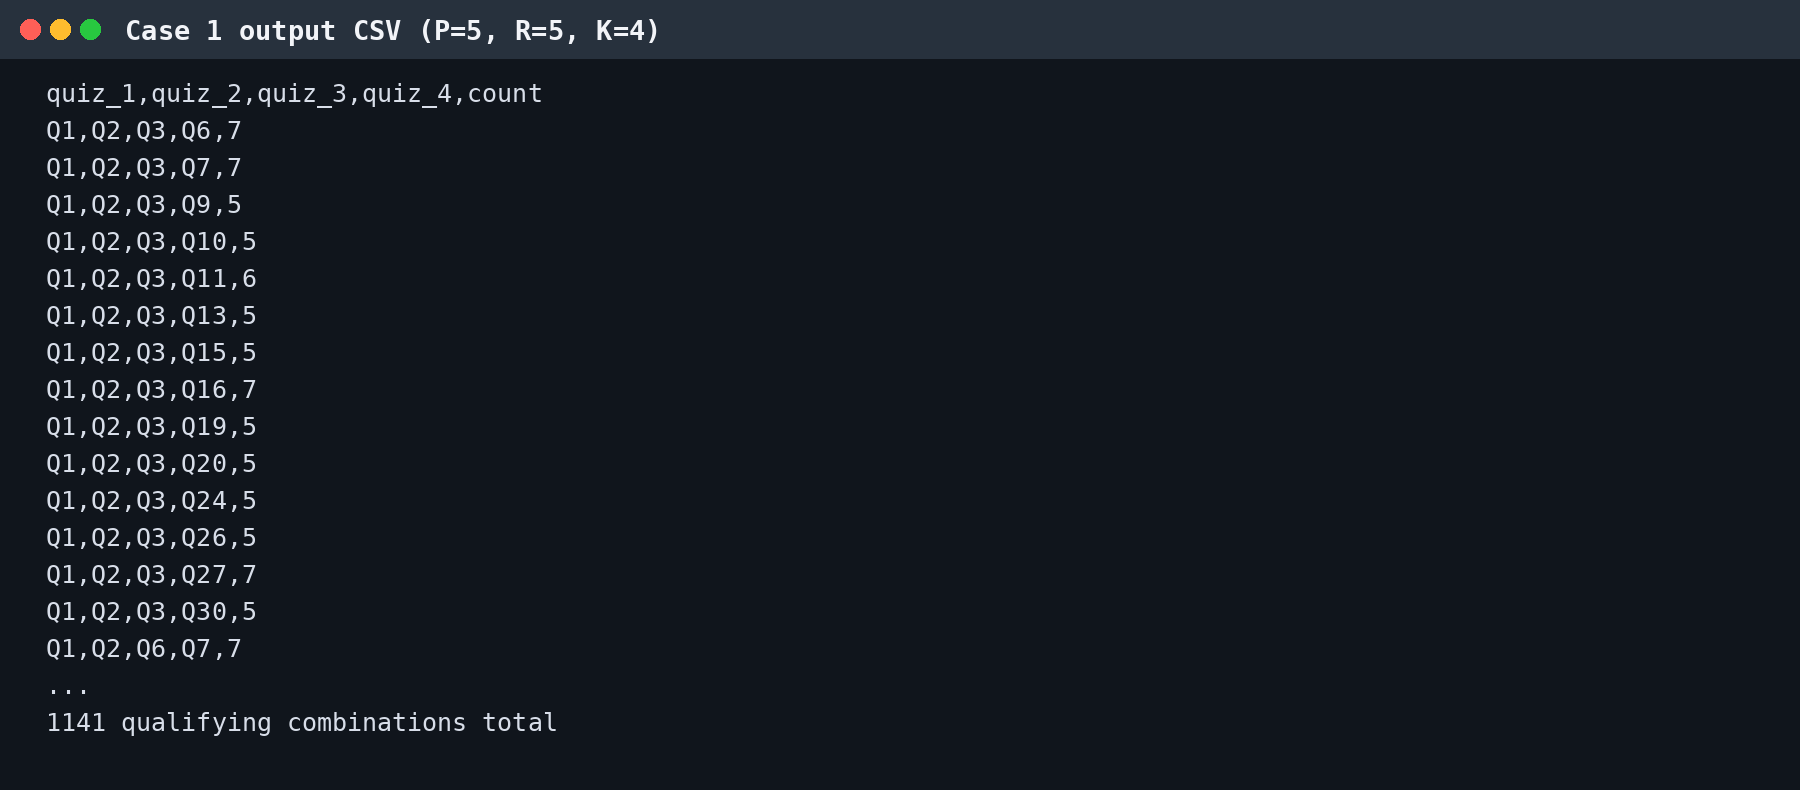
\includegraphics[width=0.96\textwidth]{../report_assets/output_case1.png}
  \caption{Beginning of the Case 1 output file. Each row is a unique ordered representation of an unordered combination.}
\end{figure}

\section{Step 4: Runtime Comparison and Asymptotic Analysis}

\subsection{Algorithm 1}
There are $\binom{N}{K}$ candidate quiz combinations. Testing one candidate requires checking $K$ scores for each of $M$ students, giving
\[
T_1(M,N,K)=\Theta\!\left(MK\binom{N}{K}\right).
\]
For fixed $K$, this is $\Theta(MN^K)$. Ignoring the required input and output storage, the temporary working space is $\Theta(MN)$ for the Boolean matrix plus $O(K)$ for one combination. If $L$ combinations qualify, storing the output adds $\Theta(LK)$.

\subsection{Algorithm 2}
Creating the singleton student sets costs $\Theta(MN)$. Let $A_d$ be the number of size-$d$ combinations whose student sets are actually constructed. With set intersections bounded by $O(M)$, a data-sensitive bound is
\[
T_2(M,N,K)=O\!\left(MN+M\sum_{d=2}^{K}A_d\right),
\qquad A_d\le\binom{N}{d}.
\]
In the worst case, every intermediate combination survives, so
\[
T_2=O\!\left(M\sum_{d=1}^{K}\binom{N}{d}\right),
\]
which is also $O(MN^K)$ for fixed $K$. Thus, Algorithm~2 does not remove the combinatorial worst case. Its practical advantage is that selective thresholds make $A_d$ much smaller than $\binom{N}{d}$ at deeper levels. Python's hash-set intersection also processes only the retained student IDs rather than rescanning the entire score row for every full combination. The implementation holds only the current and next levels, giving worst-case temporary space $O\bigl(M\max_{d\le K}\binom{N}{d}\bigr)$, in addition to input and output.

\subsection{Interpretation}
Algorithm~1's runtime changed little between cases because it always tests all $\binom{30}{4}=27{,}405$ four-quiz combinations against all students. Algorithm~2 responded to selectivity: in Case 2, only 522 three-quiz combinations survived to generate 268 final combinations. This explains why its speedup rose from 24.41$\times$ to 68.62$\times$. Algorithm~1 is simpler and is a strong validation oracle for small inputs. Algorithm~2 is preferred for interactive queries when $P$ and $R$ prune a substantial portion of the search space.

\section{Step 5: AI-Assisted Exploration}

\subsection{ChatGPT prompt and response}
\textbf{Model used:} ChatGPT, GPT-5 family, accessed September 2026.

The prompt asked the model to design both exhaustive and stepwise solutions, keep all problem dimensions general, avoid an external database, and explain correctness, pruning, data structures, and complexity. Figure~\ref{fig:chatgpt} records the prompt and response used for this work.

\begin{figure}[H]
  \centering
  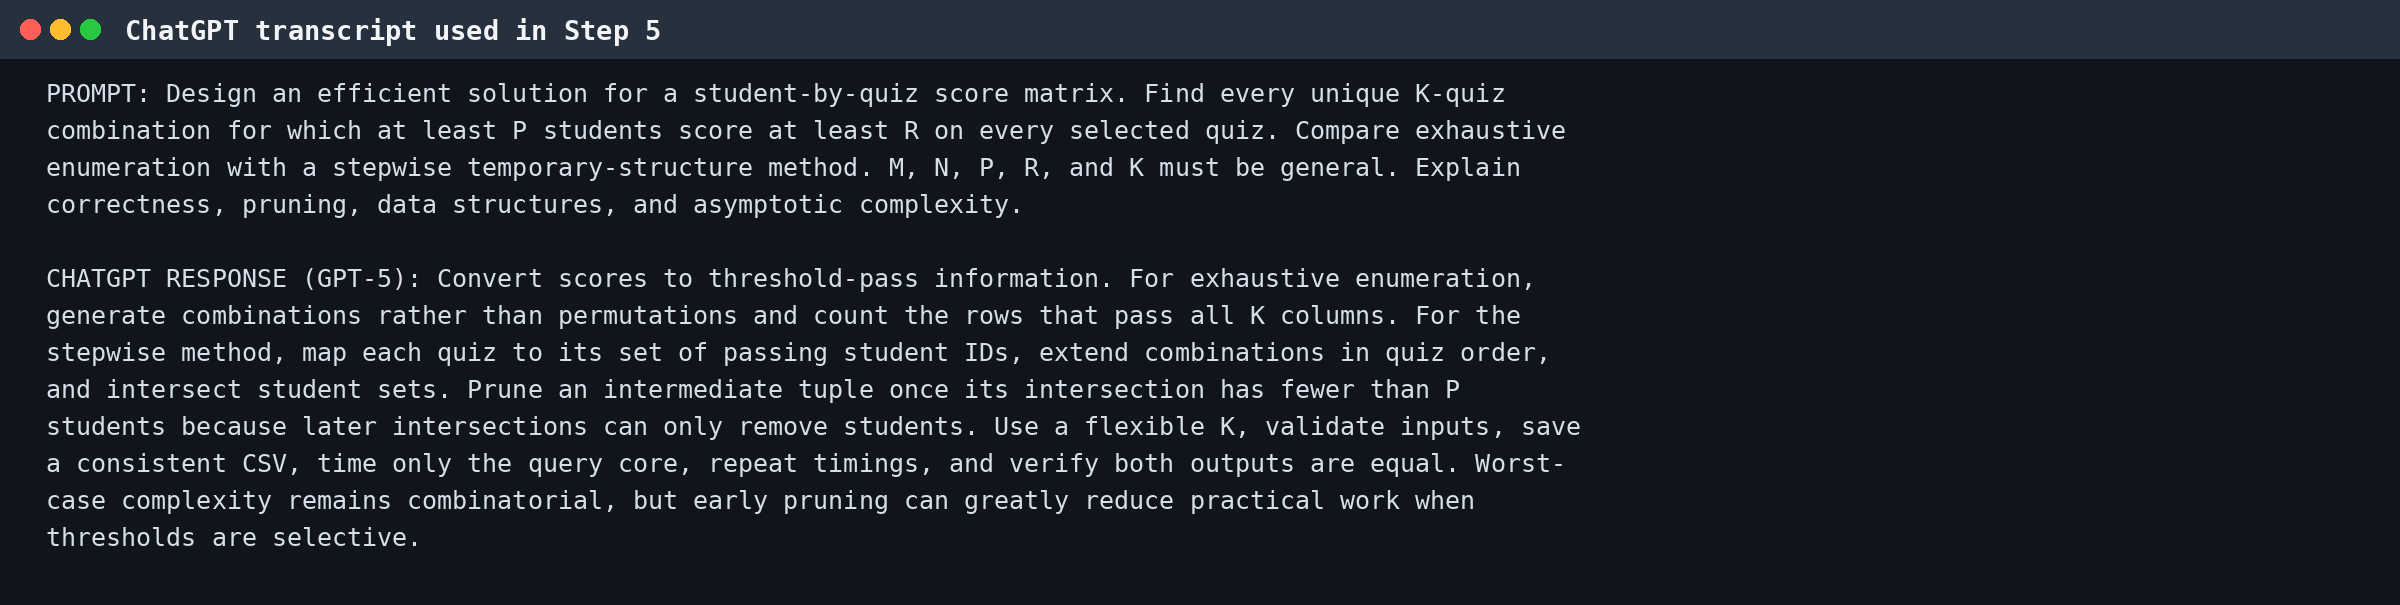
\includegraphics[width=\textwidth]{../report_assets/chatgpt_transcript.png}
  \caption{ChatGPT prompt and response transcript.}
  \label{fig:chatgpt}
\end{figure}

The most useful suggestions were: (1) use combinations rather than permutations to remove duplicates; (2) threshold the scores once; (3) represent each quiz by a qualifying-student set; (4) justify early pruning using the fact that intersections can only shrink; (5) generalize the combination size to $K$; and (6) verify the optimized output against the exhaustive baseline. These recommendations are consistent with the final implementation. Repeating timings and reporting a median also made the practical comparison more defensible.

\subsection{Second AI model prompt and required evidence}
The exact prompt for the second model is included as \texttt{second\_ai\_prompt.txt}. It should be run without modification in Gemini or Grok so the comparison uses the same task statement.

\todoBox{Run \texttt{second\_ai\_prompt.txt} in Gemini or Grok. Insert a real screenshot below, record the model/version and access date, and replace the bracketed comparison statements with observations supported by that response. Do not submit invented AI evidence.}

\begin{center}
\fbox{\parbox[c][2.0in][c]{0.88\textwidth}{\centering
\textbf{INSERT SECOND-AI SCREENSHOT HERE}\\[0.5em]
Suggested filename: \texttt{second\_ai\_response.png}}}
\end{center}

\textbf{Second model used:} [Gemini/Grok and exact version]\\
\textbf{Access date:} [date]\\
\textbf{Suggestions that made sense:} [Summarize the second model's useful recommendations and connect them to the implemented algorithms.]\\

\textbf{Comparison:} Both ChatGPT and [second model] recognized [verified common suggestions]. ChatGPT placed more emphasis on [verify from the responses], whereas [second model] emphasized [verify from the responses]. [State whether either response contained an incorrect, unnecessary, or especially useful suggestion.]\\

\textbf{Preferred method/model:} For the implemented solution, Algorithm~2 is preferred because it preserves exactness while pruning candidates that cannot meet $P$. Among the AI responses, [choose ChatGPT or the second model] was more useful because [give a concrete, response-based reason].

\section{Conclusion}
Both programs correctly identify all nonredundant quiz combinations meeting the student-count and score thresholds. Exhaustive enumeration is direct and useful as a reference implementation, but its work is insensitive to threshold selectivity. Stepwise filtering exploits anti-monotone student-set intersections and was 24.41--68.62 times faster on the two reproducible test cases. Its worst case remains combinatorial, yet it is the better practical choice for real-time queries when early levels can be pruned. The code is general with respect to $M$, $N$, $P$, $R$, and $K$, and its regression tests confirm agreement between the two methods.

\appendix
\section{Submitted Source Files}
\small
\begin{itemize}[leftmargin=*,nosep]
  \item \texttt{data\_generate.py}: reproducible CSV generator.
  \item \texttt{algorithm1.py}: exhaustive enumeration.
  \item \texttt{algorithm2.py}: general stepwise filtering from level 1 through $K$.
  \item \texttt{quiz\_query\_common.py}: shared validation and CSV writing.
  \item \texttt{run\_experiments.py}: two test cases, repeated timings, and equality check.
  \item \texttt{test\_algorithms.py}: 100 additional cross-method regression cases.
  \item \texttt{requirements.txt} and \texttt{README.md}: dependencies and commands.
  \item \texttt{second\_ai\_prompt.txt}: identical prompt for the required second model.
\end{itemize}
\normalsize

\end{document}
